\documentclass[12pt]{book}

%These tell TeX which packages to use.
\usepackage{array,epsfig}
\usepackage{amsmath}
\usepackage{amsfonts}
\usepackage{amssymb}
\usepackage{amsxtra}
\usepackage{amsthm}
\usepackage{mathrsfs}
\usepackage{color}
\usepackage{eurosym}
\usepackage{times}
\usepackage{enumitem}
\usepackage[normalem]{ulem}

%Here I define some theorem styles and shortcut commands for symbols I use often
\theoremstyle{definition}
\newtheorem{defn}{Definition}
\newtheorem{thm}{Theorem}
\newtheorem{cor}{Corollary}
\newtheorem*{rmk}{Remark}
\newtheorem{lem}{Lemma}
\newtheorem*{joke}{Joke}
\newtheorem{ex}{Example}
\newtheorem*{soln}{Solution}
\newtheorem{prop}{Proposition}

\newcommand{\lra}{\longrightarrow}
\newcommand{\ra}{\rightarrow}
\newcommand{\surj}{\twoheadrightarrow}
\newcommand{\graph}{\mathrm{graph}}
\newcommand{\bb}[1]{\mathbb{#1}}
\newcommand{\Z}{\bb{Z}}
\newcommand{\Q}{\bb{Q}}
\newcommand{\R}{\bb{R}}
\newcommand{\C}{\bb{C}}
\newcommand{\N}{\bb{N}}
\newcommand{\M}{\mathbf{M}}
\newcommand{\m}{\mathbf{m}}
\newcommand{\MM}{\mathscr{M}}
\newcommand{\HH}{\mathscr{H}}
\newcommand{\Om}{\Omega}
\newcommand{\Ho}{\in\HH(\Om)}
\newcommand{\bd}{\partial}
\newcommand{\del}{\partial}
\newcommand{\bardel}{\overline\partial}
\newcommand{\textdf}[1]{\textbf{\textsf{#1}}\index{#1}}
\newcommand{\img}{\mathrm{omega}}
\newcommand{\ip}[2]{\left\langle{#1},{#2}\right\rangle}
\newcommand{\inter}[1]{\mathrm{int}{#1}}
\newcommand{\exter}[1]{\mathrm{ext}{#1}}
\newcommand{\cl}[1]{\mathrm{cl}{#1}}
\newcommand{\ds}{\displaystyle}
\newcommand{\vol}{\mathrm{vol}}
\newcommand{\cnt}{\mathrm{ct}}
\newcommand{\osc}{\mathrm{osc}}
\newcommand{\LL}{\mathbf{L}}
\newcommand{\UU}{\mathbf{U}}
\newcommand{\support}{\mathrm{support}}
\newcommand{\AND}{\;\wedge\;}
\newcommand{\OR}{\;\vee\;}
\newcommand{\Oset}{\varnothing}
\newcommand{\st}{\ni}
\newcommand{\wh}{\widehat}

%Pagination stuff.
\setlength{\topmargin}{-.3 in}
\setlength{\oddsidemargin}{0in}
\setlength{\evensidemargin}{0in}
\setlength{\textheight}{9.in}
\setlength{\textwidth}{6.5in}
\pagestyle{empty}

\begin{document}

\begin{center}
{\Large DATA 221 \\  Homework 2  }\\
\textbf{ Trimble}\\ %You should put your name here
Due: 11:59pm  Friday 2023-04-07 
\end{center}

\vspace{0.2 cm}

\subsection*{   }

\begin{enumerate}

%\item
%Generate artificial data drawn from three classes, each a bivariate normal distribution, with the following parameters:
%
%\begin{tabular}{cccccccc}
%Class &  $x_0$  & $y_0$ & $\sigma_{xx}$ & $\sigma_{yy}$ & $\sigma_{xy}$ & n  \\
%Class A & -2 & 3 & 1 & 1.3 & 0.34 & 60\\
%Class B & 2 & -3 & 1 & 1.3 & 0.34 & 100 \\
%Class C & 0 & 0 & 0.7 & 0.7l &0.7 & 20 \\
%\end{tabular}

%In other words, draw a sample of 200 $(x,y)$ pairs, each with a label for class A, B, or C.
%Plot these on a scatter plot.

\item


\textbf{Naive Bayesian Spam Classifier}

This problem asks you to build a function to estimate the (posterior) probability that an SMS message is spam based on the words (or some subset of the words) that it contains.

The UCI "SMS Spam Collection Dataset" submitted by Almeida and Hidalgo,  is a collection of 5000 text messages, 13\% of which are labeled as spam.  Tokenize and count the word usage for the spam messages and the word usages for the ham messages.

% \texttt{https://www.kaggle.com/datasets/uciml/sms-spam-collection-dataset/}
\texttt{https://archive.ics.uci.edu/ml/datasets/sms+spam+collection}

Construct a function that scores new text messages by estimating $ {P (spam ) \over P(ham) } $ by taking some function of the empirical word frequencies in the dataset $P (word | ham)$ and $P( word | spam ) $ 

This is an ill-posed problem.  We have to decide how to handle words that are absent from one (or the other) dataset, words with small numbers of occurrances, and decide how many words to use.   Describe your choices briefly.

To prevent our model from gettig carried away, let's limit the influence of any word to a factor of $\pm$ log(100) in log-odds score:  a message of 4 words that only appear in the spam corpus will get a score of 100,000,000:1, and an utterance of 2 words that appear only in the ham corpus would get 1:10,000.  

\begin{enumerate}[label=(\alph*)]
\item Split the UCI corpus into a training and a testing dataset, say, 90/10, train the model on the 90\%.

\item Evaluate and report the confusion matrix after running the classifer on the testing subset (about 50 spam and 400 non-spam).

\item
Score all of the messages in the "testing" corpus compiled by Mohammed Noor Hassan in 

\texttt{https://github.com/mohammadnoorulhasan/sms-spam-prediction \\
/blob/master/Problem/Testing.csv}

and plot the histogram of log-odds-scores of messages (disaggregated by Spam /not spam).  Plot the histogram of probabilities for these messages.

Example code for tokenization will be provided.  You might recognize this as a variant of the loaded dice problem; words are the outcome of a dice with 50,000 sides.

\end{enumerate}
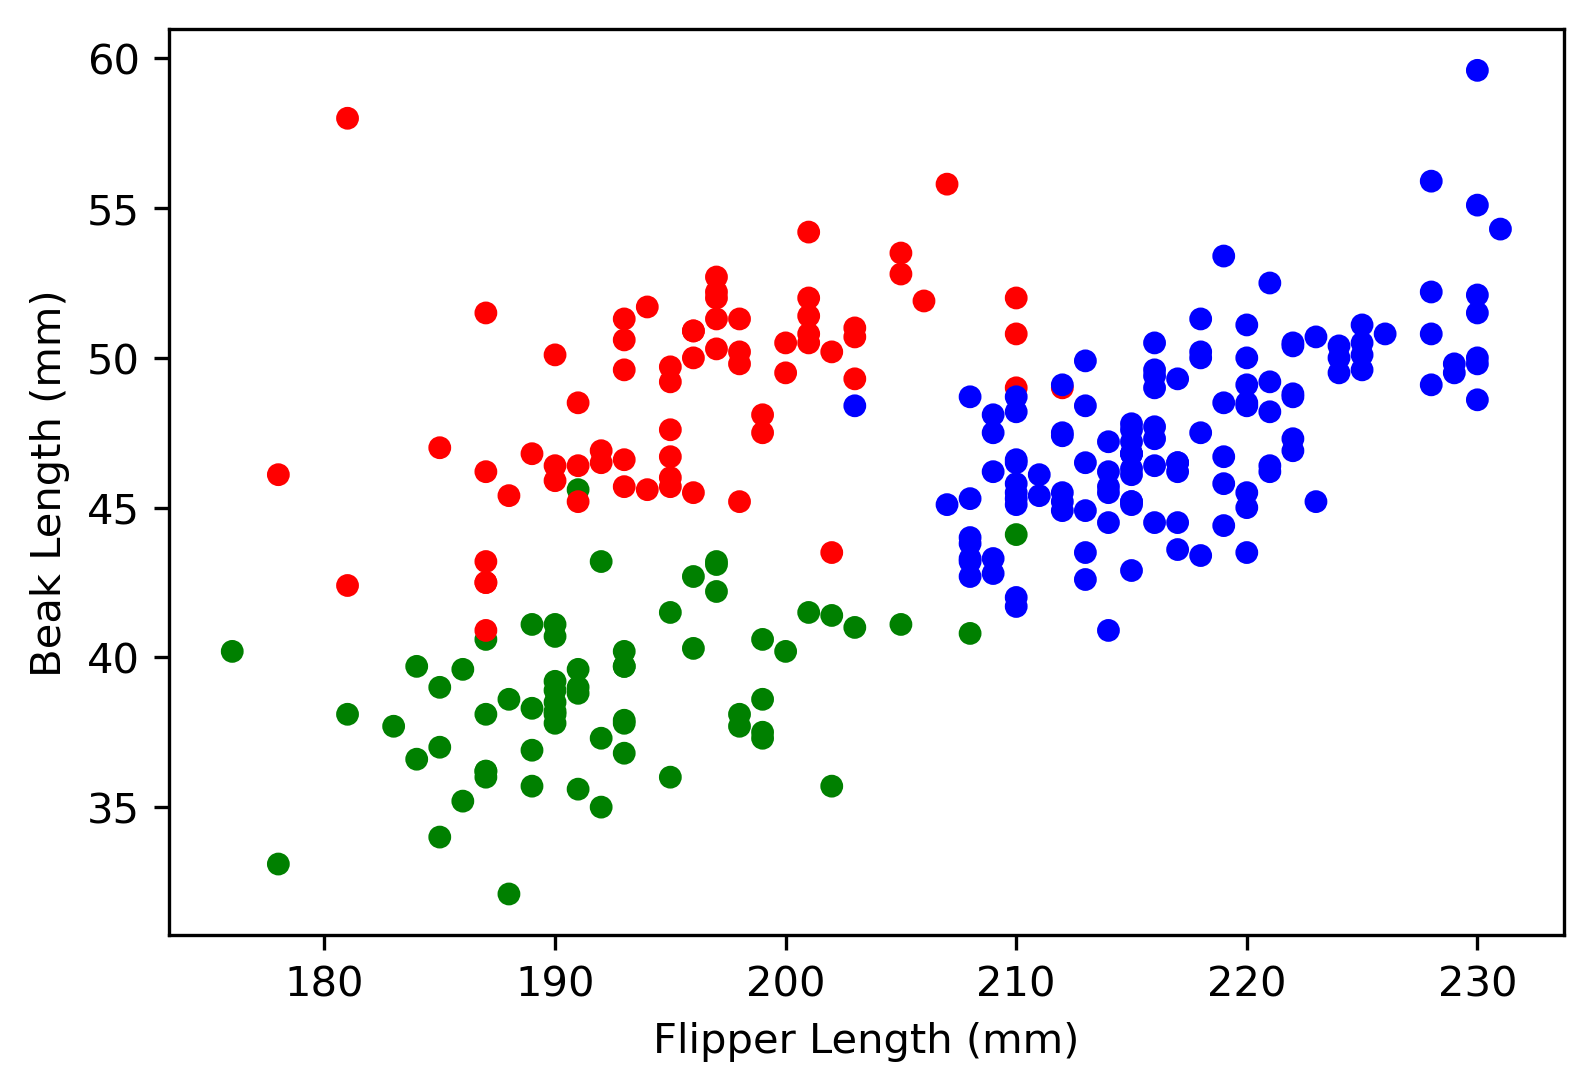
\includegraphics[width=4in]{PENGUIN.png}

\item\label{penguin}
\textbf{Linear Regression, Logistic Regression, and Linear Discriminant Analysis }
This dataset has two "label" variables (sex and species) and four numerical "features."   We will try to classify penguins by species using three techniques that look at linear combinations of the feature vectors.
\begin{enumerate}[label=(\alph*)]
\item 
As before, split the dataset into training and testing subsets.  Maybe 80/20 this time, we don't want to run out of penguins.

\item
Find logistic regression coefficents to classify penguins by sex using the four four-dimensional X (flipper length, beak width, beak length, and mass). 

\item
Classify the test set by sex and report the confusion matrix.

\item
Find logistic regression coefficents for the indicator variables for species identity against the four-dimensional X.  
Plot the decision boundaries between the classes implied by the regression coefficients on top of the scatter plot.  This requires a little bit of algebra.

\item
Find logistic regression coefficents for the indicator variables for species identity against the four-dimensional X + sex indicator variable. 

\item
Classify the test set by species and report the confusion matrix for both of the classification methods above.

Here you can either plot the boundaries by finding the equations for the boundary or, if you find it easier, evaluate a classifier at a few hundred points on a 2d grid and plot a symbol on the graph indicating which regions of X get which classification; you can solve this with math or you can solve it numerically.  
\end{enumerate}


% \item\label{normal}
% \textbf{\sout{Bivariate normal properties NO NO NO }}
% Given a two-dimensional multivariate Gaussian distribution centered on (0,0) : 

%$$ \mathcal{N} ( \mathbf{x} ; \mathbf{\Sigma} ) =
%{ 1 \over( 2 \pi  ) }  
%{ 1 \over ( \sigma_{11}^2\sigma_{22}^2 - \sigma_{12}^2 )   }
%\exp  - { 1 \over 2} (
%\begin{bmatrix}
%x_0, & x_1
%\end{bmatrix}
%\begin{bmatrix}
%\sigma_{11}^2 & \sigma_{12}^2\\
%\sigma_{12}^2 & \sigma_{22}^2
%\end{bmatrix}^{-1}
%\begin{bmatrix}
%x_0 \\
%x_1
%\end{bmatrix} ) $$

%There are two linear combinations of $x_1$ and $x_2$ that maximize (minimize) the variance of the sums
%and at the same time make the two sums independent of each other.

%We can parameterize all possible sums of f $x_1$ and $x_2$  with $\theta$ : 

%$e_1 = \begin{pmatrix} 
%cos \theta \\
%sin \theta   \\
%\end{pmatrix} $ 
%and 
% $e_2 = \begin{pmatrix} 
%-sin \theta \\
%cos \theta   \\
%\end{pmatrix} $ 

%$$ z_1 = e_1 \cdot x $$
%and
%$$ z_2 = e_2 \cdot x $$
%Find the value of $\theta$ which makes the covariance between  $z_1$ and $z_2$ vanish.  Find the standard deviations of $z_1$ and $z_2$.



\end{enumerate}
\end{document}


